\section{问题分析}

四问共享同一物理对象与同一套输运机理，差别只在物性关系、终止判据与求解域是否随时间变化。
公共连续模型与离散方法前置，各问只陈述新增内容，依赖次序见图~\ref{fig:roadmap}。

\begin{figure}[H]
  \centering
  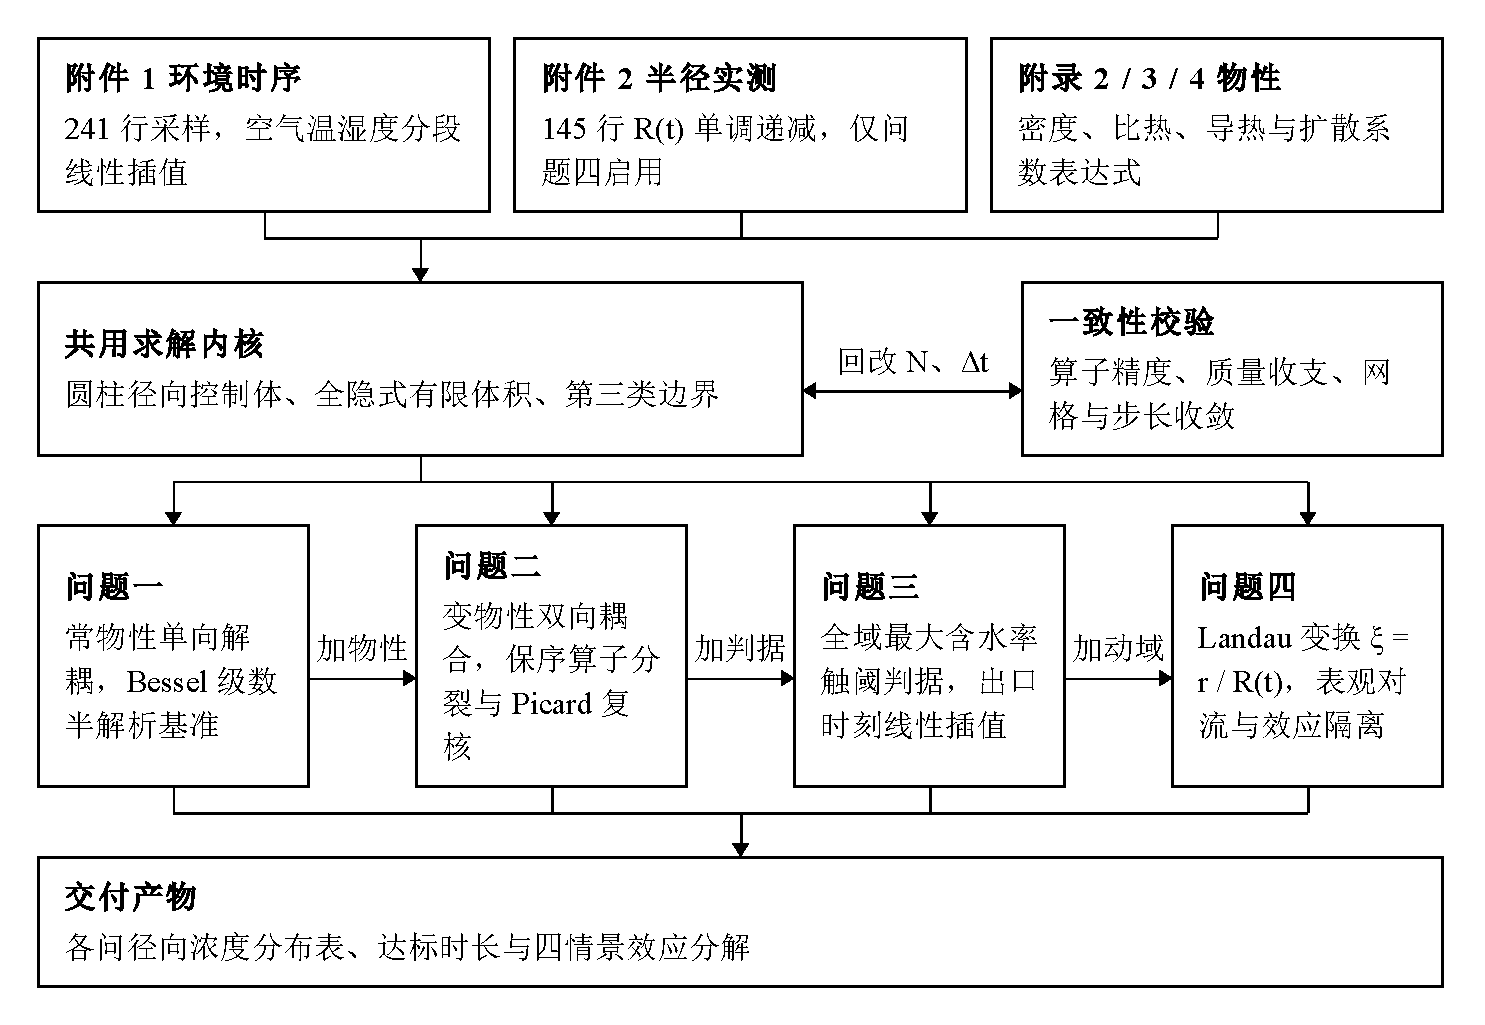
\includegraphics[width=0.92\textwidth,height=0.42\textheight,keepaspectratio]{../figures/fig_roadmap.pdf}
  \caption{全文建模路线}
  \label{fig:roadmap}
\end{figure}

题给三份材料汇入同一求解内核；一致性校验不达标时回改的是控制体数与时间步长，而不是物性。
四问呈链式而非并列排布，因为每一问只新增一项机制。两场耦合结构见图~\ref{fig:coupling_structure}。

\subsection{问题一的分析}

本问是给定环境驱动下的瞬态输运正问题。热扩散明显快于质扩散，表面与内部阻力均不可忽略，
因此采用柱坐标分布参数模型与第三类边界；具体倍数与毕奥数见问题一的半解析校核。
集中参数会抹去径向差异。常物性下温度场可用 Bessel 级数配合 Duhamel 叠加得到半解析解，
这是全题唯一可与数值解独立比对的外部数学基准。

\subsection{问题二的分析}

放开物性后任务类型不变而数学类型改变。密度、比热容、导热系数随含水率变化，使能量方程
系数由水分场决定；水分扩散系数含绝对温度指数因子，使水分方程系数由温度场决定。
两场构成双向耦合环，不能先算完整条温度时程再算水分。附录 2 下两条耦合边同时断开；
附录 3 与附录 4 下必须同步推进。物性取用哪一层场、耦合如何收敛，见公共模型。

\subsection{问题三的分析}

模型结构不改，只追加事件型终止条件。含水率沿半径始终中心最高、表面最低；以体平均判定
会在芯部尚未达标时提前结束。本文把达标时刻定义为逐点最大含水率首次达到阈值的时刻，
并在输出步之间插值定位。两种判据的量化差别见结果部分。

\subsection{问题四的分析}

本问同时更换附录 4 物性并引入径向收缩。干基含水率是物质点上的场；直接在物理坐标上离散
需每步重构网格。仿射收缩下取 $\xi=r/R(t)$（等价 $\eta=(r/R)^2$），计算域固定，主闭合不再含
表观对流。直接比较问题三、四时长并归因于「收缩加快干燥」会混淆两项改动，故用单因素情景链
把净差拆成换物性与加收缩。附录 4 密度关系与附件 2 半径在干物质守恒下并不完全相容，
该不相容度只作诊断，不修正实测半径。
